\section{Programming details}

\subsection{Programming language}
The routines developed for this project was done using the Python programming language.
The SciPy and NumPy modules provide the majority of the mathematical functions used.

\subsection{Qhull}\label{sec:qhull}
Extensive use is made of the \qhull algorithm \citep{qhull} for the calculation of normals, vertices and hypervolumes.
This algorithm was selected on the basis of its multidimentional functionality and the availability of Unix binaries.
Other Python libraries were considered but deemed insufficient, the most prominent routines being:
\begin{itemize}
\item The \texttt{spatial} module of SciPy contains a Python implementation of the \qhull algorithm but does not currently allow for volume and normal calculation.
\item The CGAL-Python project \citep{cgal} provides Python bindings to the Computational Geometry Algorithms Library (CGAL) but does not support more than 3 dimensions.
\end{itemize}

For this project, the \qhull algorithm is directly implemented from its Unix binaries.
A Python subprocess call is used and communication with \qhull is done through standard input and standard output.
The \qhull algorithm works with vertices and conversion between vertices and half-spaces are done throughout the code.

\subsection{Constraint set class}
\label{sec:conclass}
A Python class, \texttt{ConSet}, was created to handle constraint sets.
Commonly used attributes of constraint sets were added as properties of the class and commonly used operations were added as methods.

\subsubsection{Constructors}
Constraint sets can be constructed from the set of constraints or from the vertices of their feasible region.
For construction from vertices, the set is assumed to be closed and the corresponding constraints are generated accordingly.
Open sets can occur when constructing from constraints as the half-spaces comprising the set are predefined.
Open sets are flagged as erroneous and construction does not proceed.

\subsubsection{Methods}
The methods of the \texttt{ConSet} class are briefly discussed below.

\heading{Volume}
The \qhull algorithm is used to calculate the hypervolume of the constraint set.
%% MEMOIZE VOLUME and expand

\heading{Space conversion}
The process model is used when converting from the input space to the output space (or vice versa).
When using a steady-state model (real matrix of gains) this results in a matrix multiplication.
Therefore, the output of this operation is a linear transformation of the vertices of the initial constraint set.

Since the steady-state gain model of the system is used steady-state information is lost, and the result of the matrix multiplication is a change in outputs (e.g. $\Delta\vect{u}$).
The nominal operating point (around which the model was linearised) is therefore specified and used to translate the change in the output space to absolute values.
For the case where only sections of a space are converted (e.g. intersections), the deviation from the nominal operating point is transformed and added to the final translation.  

\heading{Intersections}
When the intersection of two constraint sets need to be calculated (as is the case with the AOS and the DOS), a method of superfluous constraints is used.

In an attempt to avoid the problem of degeneracy (dissertation section~\ref{M-sec:hgeometry}) the constraints that define the intersection are preprocessed.
Redundant constraints are removed or retained according to the following criteria:
\begin{itemize}
\item Co-planar (duplicate) constraints will appear in the final solution and are retained.
\item If all the vertices (of both intersecting sets) satisfy a given constraint, and a duplicate thereof does not exist, then that constraint is degenerate and excluded from the solution.
\item If only a subset of the vertices violate a given constraint, then no verdict can be made about its degeneracy.
\end{itemize}
The final retained constraints of both sets are combined into a single set, the feasible region of this set represents the intersection of the two initial sets.

\heading{Constraint reformatting}
The \texttt{ConSet} class allows for constraint sets to be expressed as a set of upper and lower limits.
The output is a reformatted $A$ matrix and $\vect{b}$ vector along with the corresponding transformations for the added variables.

\heading{Checks}
A check to determine whether one constraint set is contained within another was added to the class.
The \texttt{allinside} method checks whether all vertices of a constraint set satisfy the constraints of another set.
With the enforcement of convexity, this is a sufficient test to ensure that the set is indeed contained.

When a set is not contained within another set, a measure to quantify the containment of the outer set is generated.
For each constraint of the outer set, the perpendicular distance of all vertices violating that constraint is calculated and summed.

\subsection{Constraint and vertex conversions}\label{sec:con2vert}
As mentioned in section~\ref{sec:qhull}, most calculations are done using the vertices of a constraint set.
Methods to convert from vertices to constraints (and vice versa) are included in this program.

For conversion from vertices to constraints, the normals of the convex hull of the set of vertices are calculated.
These normals satisfy $A\vect{x} \leq -\vect{b}$ \citep{qhulldocs} and from this the constraints can be calculated directly.

The conversion from constraints to vertices is slightly more complex.
Matlab code by \citet{con2vert} was converted to Python code.
This code employs a primal-dual polytope method to calculate the resulting vertices.
This method can produce duplicate vertices; the output is therefore checked and duplicates removed.
% Add math reference

\subsection{Constraint set fitting}\label{sec:confit}
\subsubsection{Facet formulation}
The minimization problem formulated in the dissertation is reviewed in equation~\ref{eq:arbvolmin} below.
\begin{align}
  \label{eq:arbvolmin}
    \min_{A,~\vect{b}}~~&\text{-volume}_{P_i}\\
    \text{s.t.}~~~~ &P_i \subset P_o \notag \\
                    &P_i \text{~and~} P_o \text{~convex} \notag
\end{align}

This formulation is based on the facets of $P_i$, with $A$ and $\vect{b}$ as the input variables for the minimization.
From these two variables the vertices of $P_i$ are calculated and subsequently the volume.

The advantages of using this formulation are:
\begin{itemize}
\item It is a more rigorous approach, as the constraints that comprise the set are actively changed to find the optimum.
\item By fixing the sizes of $A$ and $\vect{b}$, the specified number of constraints to fit is ensured.
\item With the use of only linear constraints, the convexity of $P_i$ is ensured.
This results from the feasible region of half-spaces being strictly convex.
\end{itemize}

This formulation, although rigorous, suffers from some problems in execution:
\begin{itemize}
\item Inconsistent gradient information is generated when checking if $P_i$ is inside $P_o$.
This arises from the fact that the concept of being `inside' one another is not defined for two half-spaces (with the exception of parallel half-spaces).
\item Superfluous degrees of freedom are present, as the complete $A$ matrix and $\vect{b}$ are solved for.
There is effectively 1 false degree of freedom for each facet of $P_i$.
The rationale for still using this formulation is simple -- full control of the $A$ matrix allows for all orientations of hyperplanes to be expressed without the use of infinite slopes.
\item Due to $A$ and $\vect{b}$ begin fully changeable, shape inversion can occur.
This occurs when constraints move in such a way that an open set is generated.
Figure~\ref{fig:shapeinversion} illustrates this concept.
\item A scaling-type problem presents itself with the calculation of the volume of $P_i$.
This comes from the fact that the volume of $P_i$ is the same for $[A,~ \vect{b}]$ and $[zA,~z\vect{b}]$ where $z\in \mathbb{R}$.
Very large elements in the rows of $A$ (and their corresponding elements in $\vect{b}$) dramatically reduces the sensitivity of objective functions.
This problem can, however, be overcome by adding a constraint to the solver used to keep the norm of $\vect{b}$ at a set value.
\end{itemize}

\begin{figure}[htbp]
  \centering
%  \includegraphics[width=8cm]{graph/shapeinversion}
  \scalebox{1}{% Graphic for TeX using PGF
% Title: /home/andre/GIT Repos/AHCampher_thesis/diagrams/shapeinversion.dia
% Creator: Dia v0.97.1
% CreationDate: Thu Jan  6 17:49:33 2011
% For: andre
% \usepackage{tikz}
% The following commands are not supported in PSTricks at present
% We define them conditionally, so when they are implemented,
% this pgf file will use them.
\ifx\du\undefined
  \newlength{\du}
\fi
\setlength{\du}{15\unitlength}
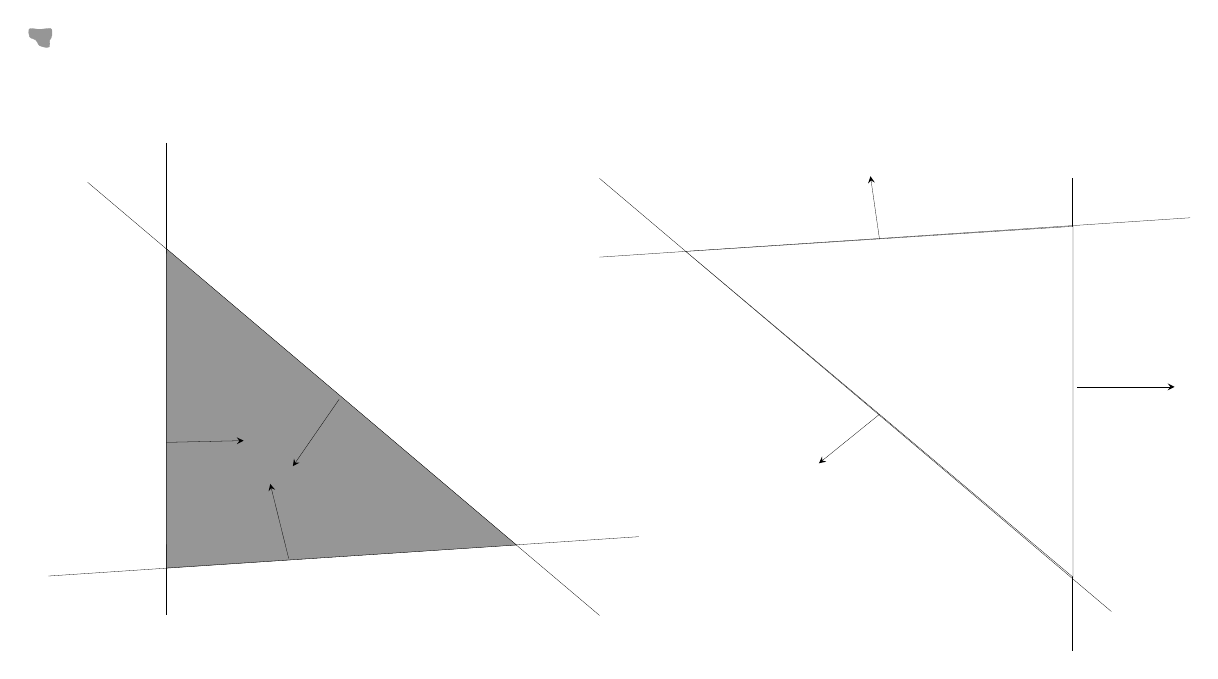
\begin{tikzpicture}
\pgftransformxscale{1.000000}
\pgftransformyscale{-1.000000}
\definecolor{dialinecolor}{rgb}{0.000000, 0.000000, 0.000000}
\pgfsetstrokecolor{dialinecolor}
\definecolor{dialinecolor}{rgb}{1.000000, 1.000000, 1.000000}
\pgfsetfillcolor{dialinecolor}
\pgfsetlinewidth{0.100000\du}
\pgfsetdash{}{0pt}
\pgfsetdash{}{0pt}
\pgfsetmiterjoin
\pgfsetbuttcap
\definecolor{dialinecolor}{rgb}{0.588235, 0.588235, 0.588235}
\pgfsetfillcolor{dialinecolor}
\pgfpathmoveto{\pgfpoint{12.158901\du}{7.905325\du}}
\pgfpathcurveto{\pgfpoint{11.158901\du}{7.905325\du}}{\pgfpoint{10.754735\du}{7.430325\du}}{\pgfpoint{10.183901\du}{6.105325\du}}
\pgfpathcurveto{\pgfpoint{9.613068\du}{4.780325\du}}{\pgfpoint{7.488068\du}{5.105325\du}}{\pgfpoint{7.408901\du}{4.205325\du}}
\pgfpathcurveto{\pgfpoint{7.329735\du}{3.305325\du}}{\pgfpoint{6.813068\du}{2.142825\du}}{\pgfpoint{7.233901\du}{1.605325\du}}
\pgfpathcurveto{\pgfpoint{7.654735\du}{1.067825\du}}{\pgfpoint{8.892235\du}{1.451159\du}}{\pgfpoint{10.508901\du}{1.580325\du}}
\pgfpathcurveto{\pgfpoint{12.125568\du}{1.709492\du}}{\pgfpoint{14.121401\du}{1.159492\du}}{\pgfpoint{15.008901\du}{1.305325\du}}
\pgfpathcurveto{\pgfpoint{15.896401\du}{1.451159\du}}{\pgfpoint{15.383901\du}{2.959492\du}}{\pgfpoint{15.508901\du}{3.880325\du}}
\pgfpathcurveto{\pgfpoint{15.633901\du}{4.801159\du}}{\pgfpoint{14.817235\du}{4.946992\du}}{\pgfpoint{14.658901\du}{5.630325\du}}
\pgfpathcurveto{\pgfpoint{14.500568\du}{6.313659\du}}{\pgfpoint{15.117235\du}{7.309492\du}}{\pgfpoint{14.558901\du}{7.980325\du}}
\pgfpathcurveto{\pgfpoint{14.000568\du}{8.651159\du}}{\pgfpoint{13.158901\du}{7.905325\du}}{\pgfpoint{12.158901\du}{7.905325\du}}
\pgfusepath{fill}
\definecolor{dialinecolor}{rgb}{0.588235, 0.588235, 0.588235}
\pgfsetstrokecolor{dialinecolor}
\pgfpathmoveto{\pgfpoint{12.158901\du}{7.905325\du}}
\pgfpathcurveto{\pgfpoint{11.158901\du}{7.905325\du}}{\pgfpoint{10.754735\du}{7.430325\du}}{\pgfpoint{10.183901\du}{6.105325\du}}
\pgfpathcurveto{\pgfpoint{9.613068\du}{4.780325\du}}{\pgfpoint{7.488068\du}{5.105325\du}}{\pgfpoint{7.408901\du}{4.205325\du}}
\pgfpathcurveto{\pgfpoint{7.329735\du}{3.305325\du}}{\pgfpoint{6.813068\du}{2.142825\du}}{\pgfpoint{7.233901\du}{1.605325\du}}
\pgfpathcurveto{\pgfpoint{7.654735\du}{1.067825\du}}{\pgfpoint{8.892235\du}{1.451159\du}}{\pgfpoint{10.508901\du}{1.580325\du}}
\pgfpathcurveto{\pgfpoint{12.125568\du}{1.709492\du}}{\pgfpoint{14.121401\du}{1.159492\du}}{\pgfpoint{15.008901\du}{1.305325\du}}
\pgfpathcurveto{\pgfpoint{15.896401\du}{1.451159\du}}{\pgfpoint{15.383901\du}{2.959492\du}}{\pgfpoint{15.508901\du}{3.880325\du}}
\pgfpathcurveto{\pgfpoint{15.633901\du}{4.801159\du}}{\pgfpoint{14.817235\du}{4.946992\du}}{\pgfpoint{14.658901\du}{5.630325\du}}
\pgfpathcurveto{\pgfpoint{14.500568\du}{6.313659\du}}{\pgfpoint{15.117235\du}{7.309492\du}}{\pgfpoint{14.558901\du}{7.980325\du}}
\pgfpathcurveto{\pgfpoint{14.000568\du}{8.651159\du}}{\pgfpoint{13.158901\du}{7.905325\du}}{\pgfpoint{12.158901\du}{7.905325\du}}
\pgfusepath{stroke}
\pgfsetlinewidth{0.100000\du}
\pgfsetdash{}{0pt}
\pgfsetdash{}{0pt}
\pgfsetbuttcap
{
\definecolor{dialinecolor}{rgb}{0.000000, 0.000000, 0.000000}
\pgfsetfillcolor{dialinecolor}
% was here!!!
\definecolor{dialinecolor}{rgb}{0.000000, 0.000000, 0.000000}
\pgfsetstrokecolor{dialinecolor}
\draw (2.000000\du,1.500000\du)--(2.000000\du,7.500000\du);
}
\pgfsetlinewidth{0.100000\du}
\pgfsetdash{}{0pt}
\pgfsetdash{}{0pt}
\pgfsetbuttcap
{
\definecolor{dialinecolor}{rgb}{0.000000, 0.000000, 0.000000}
\pgfsetfillcolor{dialinecolor}
% was here!!!
\definecolor{dialinecolor}{rgb}{0.000000, 0.000000, 0.000000}
\pgfsetstrokecolor{dialinecolor}
\draw (1.000000\du,2.000000\du)--(7.500000\du,7.500000\du);
}
\pgfsetlinewidth{0.100000\du}
\pgfsetdash{}{0pt}
\pgfsetdash{}{0pt}
\pgfsetbuttcap
{
\definecolor{dialinecolor}{rgb}{0.000000, 0.000000, 0.000000}
\pgfsetfillcolor{dialinecolor}
% was here!!!
\definecolor{dialinecolor}{rgb}{0.000000, 0.000000, 0.000000}
\pgfsetstrokecolor{dialinecolor}
\draw (0.500000\du,7.000000\du)--(8.000000\du,6.500000\du);
}
\pgfsetlinewidth{0.100000\du}
\pgfsetdash{}{0pt}
\pgfsetdash{}{0pt}
\pgfsetbuttcap
{
\definecolor{dialinecolor}{rgb}{0.000000, 0.000000, 0.000000}
\pgfsetfillcolor{dialinecolor}
% was here!!!
\definecolor{dialinecolor}{rgb}{0.000000, 0.000000, 0.000000}
\pgfsetstrokecolor{dialinecolor}
\draw (13.500000\du,1.950000\du)--(13.500000\du,7.950000\du);
}
\pgfsetlinewidth{0.100000\du}
\pgfsetdash{}{0pt}
\pgfsetdash{}{0pt}
\pgfsetbuttcap
{
\definecolor{dialinecolor}{rgb}{0.000000, 0.000000, 0.000000}
\pgfsetfillcolor{dialinecolor}
% was here!!!
\definecolor{dialinecolor}{rgb}{0.000000, 0.000000, 0.000000}
\pgfsetstrokecolor{dialinecolor}
\draw (7.500000\du,1.950000\du)--(14.000000\du,7.450000\du);
}
\pgfsetlinewidth{0.100000\du}
\pgfsetdash{}{0pt}
\pgfsetdash{}{0pt}
\pgfsetbuttcap
{
\definecolor{dialinecolor}{rgb}{0.000000, 0.000000, 0.000000}
\pgfsetfillcolor{dialinecolor}
% was here!!!
\definecolor{dialinecolor}{rgb}{0.000000, 0.000000, 0.000000}
\pgfsetstrokecolor{dialinecolor}
\draw (7.500000\du,2.950000\du)--(15.000000\du,2.450000\du);
}
\pgfsetlinewidth{0.100000\du}
\pgfsetdash{}{0pt}
\pgfsetdash{}{0pt}
\pgfsetmiterjoin
\pgfsetbuttcap
\definecolor{dialinecolor}{rgb}{0.588235, 0.588235, 0.588235}
\pgfsetfillcolor{dialinecolor}
\fill (2.000781\du,2.843133\du)--(6.445313\du,6.605633\du)--(1.999219\du,6.897821\du)--cycle;
\definecolor{dialinecolor}{rgb}{0.000000, 0.000000, 0.000000}
\pgfsetstrokecolor{dialinecolor}
\draw (2.000781\du,2.843133\du)--(6.445313\du,6.605633\du)--(1.999219\du,6.897821\du)--cycle;
\pgfsetlinewidth{0.100000\du}
\pgfsetdash{}{0pt}
\pgfsetdash{}{0pt}
\pgfsetmiterjoin
\pgfsetbuttcap
\definecolor{dialinecolor}{rgb}{1.000000, 1.000000, 1.000000}
\pgfsetfillcolor{dialinecolor}
\fill (8.596401\du,2.877508\du)--(13.514062\du,2.558758\du)--(13.514062\du,7.015008\du)--cycle;
\definecolor{dialinecolor}{rgb}{0.000000, 0.000000, 0.000000}
\pgfsetstrokecolor{dialinecolor}
\draw (8.596401\du,2.877508\du)--(13.514062\du,2.558758\du)--(13.514062\du,7.015008\du)--cycle;
\pgfsetlinewidth{0.100000\du}
\pgfsetdash{}{0pt}
\pgfsetdash{}{0pt}
\pgfsetbuttcap
{
\definecolor{dialinecolor}{rgb}{0.000000, 0.000000, 0.000000}
\pgfsetfillcolor{dialinecolor}
% was here!!!
\pgfsetarrowsend{stealth}
\definecolor{dialinecolor}{rgb}{0.000000, 0.000000, 0.000000}
\pgfsetstrokecolor{dialinecolor}
\draw (4.193276\du,4.755325\du)--(3.605776\du,5.605325\du);
}
\pgfsetlinewidth{0.100000\du}
\pgfsetdash{}{0pt}
\pgfsetdash{}{0pt}
\pgfsetbuttcap
{
\definecolor{dialinecolor}{rgb}{0.000000, 0.000000, 0.000000}
\pgfsetfillcolor{dialinecolor}
% was here!!!
\pgfsetarrowsend{stealth}
\definecolor{dialinecolor}{rgb}{0.000000, 0.000000, 0.000000}
\pgfsetstrokecolor{dialinecolor}
\draw (11.055232\du,4.946258\du)--(10.287026\du,5.567825\du);
}
\pgfsetlinewidth{0.100000\du}
\pgfsetdash{}{0pt}
\pgfsetdash{}{0pt}
\pgfsetbuttcap
{
\definecolor{dialinecolor}{rgb}{0.000000, 0.000000, 0.000000}
\pgfsetfillcolor{dialinecolor}
% was here!!!
\pgfsetarrowsend{stealth}
\definecolor{dialinecolor}{rgb}{0.000000, 0.000000, 0.000000}
\pgfsetstrokecolor{dialinecolor}
\draw (11.055232\du,2.718133\du)--(10.940776\du,1.922129\du);
}
\pgfsetlinewidth{0.100000\du}
\pgfsetdash{}{0pt}
\pgfsetdash{}{0pt}
\pgfsetbuttcap
{
\definecolor{dialinecolor}{rgb}{0.000000, 0.000000, 0.000000}
\pgfsetfillcolor{dialinecolor}
% was here!!!
\pgfsetarrowsend{stealth}
\definecolor{dialinecolor}{rgb}{0.000000, 0.000000, 0.000000}
\pgfsetstrokecolor{dialinecolor}
\draw (3.552026\du,6.774629\du)--(3.318276\du,5.830325\du);
}
\pgfsetlinewidth{0.100000\du}
\pgfsetdash{}{0pt}
\pgfsetdash{}{0pt}
\pgfsetbuttcap
{
\definecolor{dialinecolor}{rgb}{0.000000, 0.000000, 0.000000}
\pgfsetfillcolor{dialinecolor}
% was here!!!
\pgfsetarrowsend{stealth}
\definecolor{dialinecolor}{rgb}{0.000000, 0.000000, 0.000000}
\pgfsetstrokecolor{dialinecolor}
\draw (2.000776\du,5.302129\du)--(2.980776\du,5.280325\du);
}
\pgfsetlinewidth{0.100000\du}
\pgfsetdash{}{0pt}
\pgfsetdash{}{0pt}
\pgfsetbuttcap
{
\definecolor{dialinecolor}{rgb}{0.000000, 0.000000, 0.000000}
\pgfsetfillcolor{dialinecolor}
% was here!!!
\pgfsetarrowsend{stealth}
\definecolor{dialinecolor}{rgb}{0.000000, 0.000000, 0.000000}
\pgfsetstrokecolor{dialinecolor}
\draw (13.565776\du,4.597129\du)--(14.803276\du,4.597129\du);
}
\end{tikzpicture}
}  
  \caption[Shape inversion example]{Shape inversion due to the movement of constraints (half-space normals arrows are shown with arrows).}
  \label{fig:shapeinversion}
\end{figure}

\subsubsection{Vertex formulation}
Another possibility was to express the problem in terms of the vertices of the convex hull of the constraint set.
For this formulation, equation~\ref{eq:arbvolmin} needs to be redefined in terms of the vertices, as shown in equation~\ref{eq:arbvolminverts}
\begin{align}
  \label{eq:arbvolminverts}
    \min_{\vect{v}}~~&\text{-volume}_{P_i}\\
    \text{s.t.}~~~~ &P_i \subset P_o \notag \\
                    &P_i \text{~and~} P_o \text{~convex} \notag
\end{align}
where $\vect{v}$ is all the vertices of $P_i$.
$A$ and $\vect{b}$ will now only result from the final optimised $P_i$.

The vertex based formulation has the following advantages:
\begin{itemize}
  \item This approach is more intuitive as the fitting problem, conceptually, involves moving the vertices of $P_i$ to the facets of $P_o$.
  \item Checking that $P_i$ is inside $P_o$ is now a direct operation, as vertices don't need to be calculated from $A$ and $\vect{b}$ first.
  \item When a measure of containment needs to be generated, consistent gradient information can be expressed in terms of each vertex of $P_i$.
\end{itemize}

Most of the problems with the vertex based method stems from the movement of vertices to the inside of the convex hull of $P_i$ during the solution of the problem.
These internal points are now no longer vertices, but are still considered in the optimisation.
This formulation was abandoned in this project due to the following disadvantages in its implementation:
\begin{itemize}
  \item A clear correlation between the number of vertices and the number of facets on a shape does not exist (unless some properties of the shape are given).
Figure~\ref{fig:vertsvsfaces} illustrates this concept for two 6-faceted, 3 dimensional shapes.
This is a major problem when the number of facets (constraints) on $P_i$ needs to be specified.
  \item A slightly different problem than the one mentioned above -- the number of facets on $P_i$ are determined by the final optimised vertices.
Internal points and duplicate vertices in the solution will cause the number of facets to decrease.
Therefore, specification of a set number of facets becomes nearly impossible.
  \item Enforcing convexity becomes a problem when vertices are used directly.
This is caused by the movement of vertices inside the convex hull of $P_i$.
If all points are to be vertices by definition, non-convex shapes are generated.
The use of the \qhull algorithm to calculate the volume now becomes invalid. 
  \item Another problem with internal points occurs during the calculation of the volume of $P_i$.
The perturbation of internal points have no effect on the volume (as only the convex hull is considered).
This results in decreased sensitivity of objective functions.
\end{itemize}

\begin{figure}[htbp]
  \centering
%  \includegraphics[width=8cm]{graph/vertsvsfaces}
  \scalebox{1.5}{% Graphic for TeX using PGF
% Title: /home/andre/GIT Repos/AHCampher_thesis/diagrams/vertsvsfaces.dia
% Creator: Dia v0.97.1
% CreationDate: Thu Jan  6 17:55:50 2011
% For: andre
% \usepackage{tikz}
% The following commands are not supported in PSTricks at present
% We define them conditionally, so when they are implemented,
% this pgf file will use them.
\ifx\du\undefined
  \newlength{\du}
\fi
\setlength{\du}{15\unitlength}
\begin{tikzpicture}
\pgftransformxscale{1.000000}
\pgftransformyscale{-1.000000}
\definecolor{dialinecolor}{rgb}{0.000000, 0.000000, 0.000000}
\pgfsetstrokecolor{dialinecolor}
\definecolor{dialinecolor}{rgb}{1.000000, 1.000000, 1.000000}
\pgfsetfillcolor{dialinecolor}
\pgfsetlinewidth{0.100000\du}
\pgfsetdash{}{0pt}
\pgfsetdash{}{0pt}
\pgfsetbuttcap
\pgfsetmiterjoin
\pgfsetlinewidth{0.100000\du}
\pgfsetbuttcap
\pgfsetmiterjoin
\pgfsetdash{}{0pt}
\definecolor{dialinecolor}{rgb}{1.000000, 1.000000, 1.000000}
\pgfsetfillcolor{dialinecolor}
\fill (2.500000\du,3.000000\du)--(2.500000\du,6.041667\du)--(5.443548\du,6.041667\du)--(5.443548\du,3.000000\du)--cycle;
\definecolor{dialinecolor}{rgb}{0.000000, 0.000000, 0.000000}
\pgfsetstrokecolor{dialinecolor}
\draw (2.500000\du,3.000000\du)--(2.500000\du,6.041667\du)--(5.443548\du,6.041667\du)--(5.443548\du,3.000000\du)--cycle;
\pgfsetbuttcap
\pgfsetmiterjoin
\pgfsetdash{}{0pt}
\definecolor{dialinecolor}{rgb}{0.000000, 0.000000, 0.000000}
\pgfsetstrokecolor{dialinecolor}
\draw (2.500000\du,3.000000\du)--(2.500000\du,6.041667\du)--(5.443548\du,6.041667\du)--(5.443548\du,3.000000\du)--cycle;
\pgfsetlinewidth{0.100000\du}
\pgfsetdash{}{0pt}
\pgfsetdash{}{0pt}
\pgfsetbuttcap
{
\definecolor{dialinecolor}{rgb}{0.000000, 0.000000, 0.000000}
\pgfsetfillcolor{dialinecolor}
% was here!!!
\definecolor{dialinecolor}{rgb}{0.000000, 0.000000, 0.000000}
\pgfsetstrokecolor{dialinecolor}
\draw (2.500000\du,6.041667\du)--(1.000000\du,5.000000\du);
}
\pgfsetlinewidth{0.100000\du}
\pgfsetdash{}{0pt}
\pgfsetdash{}{0pt}
\pgfsetbuttcap
{
\definecolor{dialinecolor}{rgb}{0.000000, 0.000000, 0.000000}
\pgfsetfillcolor{dialinecolor}
% was here!!!
\definecolor{dialinecolor}{rgb}{0.000000, 0.000000, 0.000000}
\pgfsetstrokecolor{dialinecolor}
\draw (2.500000\du,3.000000\du)--(1.000000\du,1.958333\du);
}
\pgfsetlinewidth{0.100000\du}
\pgfsetdash{}{0pt}
\pgfsetdash{}{0pt}
\pgfsetbuttcap
{
\definecolor{dialinecolor}{rgb}{0.000000, 0.000000, 0.000000}
\pgfsetfillcolor{dialinecolor}
% was here!!!
\definecolor{dialinecolor}{rgb}{0.000000, 0.000000, 0.000000}
\pgfsetstrokecolor{dialinecolor}
\draw (5.443548\du,3.000000\du)--(4.000000\du,1.958333\du);
}
\pgfsetlinewidth{0.100000\du}
\pgfsetdash{}{0pt}
\pgfsetdash{}{0pt}
\pgfsetbuttcap
{
\definecolor{dialinecolor}{rgb}{0.000000, 0.000000, 0.000000}
\pgfsetfillcolor{dialinecolor}
% was here!!!
\definecolor{dialinecolor}{rgb}{0.000000, 0.000000, 0.000000}
\pgfsetstrokecolor{dialinecolor}
\draw (1.000000\du,5.000000\du)--(1.000000\du,2.000000\du);
}
\pgfsetlinewidth{0.100000\du}
\pgfsetdash{}{0pt}
\pgfsetdash{}{0pt}
\pgfsetbuttcap
{
\definecolor{dialinecolor}{rgb}{0.000000, 0.000000, 0.000000}
\pgfsetfillcolor{dialinecolor}
% was here!!!
\definecolor{dialinecolor}{rgb}{0.000000, 0.000000, 0.000000}
\pgfsetstrokecolor{dialinecolor}
\draw (1.000000\du,2.000000\du)--(4.000000\du,2.000000\du);
}
\pgfsetlinewidth{0.100000\du}
\pgfsetdash{{0.200000\du}{0.200000\du}}{0\du}
\pgfsetdash{{0.200000\du}{0.200000\du}}{0\du}
\pgfsetbuttcap
{
\definecolor{dialinecolor}{rgb}{0.000000, 0.000000, 0.000000}
\pgfsetfillcolor{dialinecolor}
% was here!!!
\definecolor{dialinecolor}{rgb}{0.000000, 0.000000, 0.000000}
\pgfsetstrokecolor{dialinecolor}
\draw (5.443548\du,6.041667\du)--(4.000000\du,4.958333\du);
}
\pgfsetlinewidth{0.100000\du}
\pgfsetdash{{0.200000\du}{0.200000\du}}{0\du}
\pgfsetdash{{0.200000\du}{0.200000\du}}{0\du}
\pgfsetbuttcap
{
\definecolor{dialinecolor}{rgb}{0.000000, 0.000000, 0.000000}
\pgfsetfillcolor{dialinecolor}
% was here!!!
\definecolor{dialinecolor}{rgb}{0.000000, 0.000000, 0.000000}
\pgfsetstrokecolor{dialinecolor}
\draw (1.000000\du,5.000000\du)--(4.000000\du,5.000000\du);
}
\pgfsetlinewidth{0.100000\du}
\pgfsetdash{{0.200000\du}{0.200000\du}}{0\du}
\pgfsetdash{{0.200000\du}{0.200000\du}}{0\du}
\pgfsetbuttcap
{
\definecolor{dialinecolor}{rgb}{0.000000, 0.000000, 0.000000}
\pgfsetfillcolor{dialinecolor}
% was here!!!
\definecolor{dialinecolor}{rgb}{0.000000, 0.000000, 0.000000}
\pgfsetstrokecolor{dialinecolor}
\draw (4.000000\du,5.000000\du)--(4.000000\du,2.000000\du);
}
\pgfsetlinewidth{0.100000\du}
\pgfsetdash{}{0pt}
\pgfsetdash{}{0pt}
\pgfsetbuttcap
{
\definecolor{dialinecolor}{rgb}{0.000000, 0.000000, 0.000000}
\pgfsetfillcolor{dialinecolor}
% was here!!!
\definecolor{dialinecolor}{rgb}{0.000000, 0.000000, 0.000000}
\pgfsetstrokecolor{dialinecolor}
\draw (8.500000\du,6.000000\du)--(11.500000\du,6.000000\du);
}
\pgfsetlinewidth{0.100000\du}
\pgfsetdash{}{0pt}
\pgfsetdash{}{0pt}
\pgfsetbuttcap
{
\definecolor{dialinecolor}{rgb}{0.000000, 0.000000, 0.000000}
\pgfsetfillcolor{dialinecolor}
% was here!!!
\definecolor{dialinecolor}{rgb}{0.000000, 0.000000, 0.000000}
\pgfsetstrokecolor{dialinecolor}
\draw (11.500000\du,6.000000\du)--(12.500000\du,5.000000\du);
}
\pgfsetlinewidth{0.100000\du}
\pgfsetdash{}{0pt}
\pgfsetdash{}{0pt}
\pgfsetbuttcap
{
\definecolor{dialinecolor}{rgb}{0.000000, 0.000000, 0.000000}
\pgfsetfillcolor{dialinecolor}
% was here!!!
\definecolor{dialinecolor}{rgb}{0.000000, 0.000000, 0.000000}
\pgfsetstrokecolor{dialinecolor}
\draw (8.500000\du,6.000000\du)--(7.500000\du,5.000000\du);
}
\pgfsetlinewidth{0.100000\du}
\pgfsetdash{{0.200000\du}{0.200000\du}}{0\du}
\pgfsetdash{{0.200000\du}{0.200000\du}}{0\du}
\pgfsetbuttcap
{
\definecolor{dialinecolor}{rgb}{0.000000, 0.000000, 0.000000}
\pgfsetfillcolor{dialinecolor}
% was here!!!
\definecolor{dialinecolor}{rgb}{0.000000, 0.000000, 0.000000}
\pgfsetstrokecolor{dialinecolor}
\draw (7.500000\du,5.000000\du)--(10.000000\du,4.000000\du);
}
\pgfsetlinewidth{0.100000\du}
\pgfsetdash{{0.200000\du}{0.200000\du}}{0\du}
\pgfsetdash{{0.200000\du}{0.200000\du}}{0\du}
\pgfsetbuttcap
{
\definecolor{dialinecolor}{rgb}{0.000000, 0.000000, 0.000000}
\pgfsetfillcolor{dialinecolor}
% was here!!!
\definecolor{dialinecolor}{rgb}{0.000000, 0.000000, 0.000000}
\pgfsetstrokecolor{dialinecolor}
\draw (12.500000\du,5.000000\du)--(10.000000\du,4.000000\du);
}
\pgfsetlinewidth{0.100000\du}
\pgfsetdash{{0.200000\du}{0.200000\du}}{0\du}
\pgfsetdash{{0.200000\du}{0.200000\du}}{0\du}
\pgfsetbuttcap
{
\definecolor{dialinecolor}{rgb}{0.000000, 0.000000, 0.000000}
\pgfsetfillcolor{dialinecolor}
% was here!!!
\definecolor{dialinecolor}{rgb}{0.000000, 0.000000, 0.000000}
\pgfsetstrokecolor{dialinecolor}
\draw (10.000000\du,4.000000\du)--(10.000000\du,2.000000\du);
}
\pgfsetlinewidth{0.100000\du}
\pgfsetdash{}{0pt}
\pgfsetdash{}{0pt}
\pgfsetbuttcap
{
\definecolor{dialinecolor}{rgb}{0.000000, 0.000000, 0.000000}
\pgfsetfillcolor{dialinecolor}
% was here!!!
\definecolor{dialinecolor}{rgb}{0.000000, 0.000000, 0.000000}
\pgfsetstrokecolor{dialinecolor}
\draw (7.500000\du,5.000000\du)--(10.000000\du,2.000000\du);
}
\pgfsetlinewidth{0.100000\du}
\pgfsetdash{}{0pt}
\pgfsetdash{}{0pt}
\pgfsetbuttcap
{
\definecolor{dialinecolor}{rgb}{0.000000, 0.000000, 0.000000}
\pgfsetfillcolor{dialinecolor}
% was here!!!
\definecolor{dialinecolor}{rgb}{0.000000, 0.000000, 0.000000}
\pgfsetstrokecolor{dialinecolor}
\draw (8.500000\du,6.000000\du)--(10.000000\du,2.000000\du);
}
\pgfsetlinewidth{0.100000\du}
\pgfsetdash{}{0pt}
\pgfsetdash{}{0pt}
\pgfsetbuttcap
{
\definecolor{dialinecolor}{rgb}{0.000000, 0.000000, 0.000000}
\pgfsetfillcolor{dialinecolor}
% was here!!!
\definecolor{dialinecolor}{rgb}{0.000000, 0.000000, 0.000000}
\pgfsetstrokecolor{dialinecolor}
\draw (11.500000\du,6.000000\du)--(10.000000\du,2.000000\du);
}
\pgfsetlinewidth{0.100000\du}
\pgfsetdash{}{0pt}
\pgfsetdash{}{0pt}
\pgfsetbuttcap
{
\definecolor{dialinecolor}{rgb}{0.000000, 0.000000, 0.000000}
\pgfsetfillcolor{dialinecolor}
% was here!!!
\definecolor{dialinecolor}{rgb}{0.000000, 0.000000, 0.000000}
\pgfsetstrokecolor{dialinecolor}
\draw (12.500000\du,5.000000\du)--(10.000000\du,2.000000\du);
}
\end{tikzpicture}
}  
  \caption[The unclear correlation between number of facets and vertices]{A cube and a pentagonal pyramid in 3 dimensions -- both shapes have 6 facets, but differ in their number of vertices (8 and 6  respectively).}
  \label{fig:vertsvsfaces}
\end{figure}

\subsubsection{Optimisation}
For the solution of the problem, two optimisers (solvers) were considered.
Both are contained in the SciPy \texttt{optimize} module:
\begin{itemize}
  \item A sequential least squares quadratic programming (SLSQP) algorithm, \texttt{fmin\_slsqp}, henceforth simply referred to as SLSQP. 
This is a gradient based, constrained solver.
  \item A downhill-simplex algorithm, \texttt{fmin}, henceforth simply referred to as simplex.
This is an unconstrained solver.
\end{itemize}

\subsubsection{Objective functions}
For SLSQP a combination of equality and inequality constraints were used.
The constrained problem formulation for SLSQP is shown in equation~\ref{eq:slsqpobjfn} and follows from equation~\ref{eq:arbvolmin}.
The criteria that $P_i$ should be convex is satisfied by using linear inequalities ($A\vect{x} \leq \vect{b}$) for its construction.
The convexity of $P_o$ is assumed to be a given.
\begin{align}
  \label{eq:slsqpobjfn}
    \min_{A,~\vect{b}}~~&\text{-volume}_{P_i}\\
    \text{s.t.}~~~~ &\text{norm}(\vect{b}) = 1 \notag \\
                    &\text{vertices}_{P_i} \text{~satisfy~} (A\vect{x}\leq\vect{b})_{P_o} \notag  
\end{align}

The constraints as imposed on SLSQP are not possible for simplex.
A penalty formulation for the objective function is therefore used.
Equation~\ref{eq:fminobjfn} shows the objective function for use with simplex.
The same argument for convexity holds as with SLSQP.
\begin{align}
  \label{eq:fminobjfn}
    \min_{A,~\vect{b}}~~&\text{-volume}_{P_i} + p_A(\text{norm}(\text{distance of vertices$_{P_i}$ outside}~P_o)) + p_B(|\text{norm}(\vect{b}) - 1|)  
\end{align}
where $p_A$ and $p_B$ are penalty weights.

The same objective functions (equations~\ref{eq:slsqpobjfn} and~\ref{eq:fminobjfn}) hold for the fitting of rectangular constraint sets.
Only difference begin that $\vect{b}$ is the only input variable and $A$ has a fixed shape (as shown in equation~\ref{M-eq:recvolmin} in the dissertation).

\subsubsection{Shape exceptions}
Two types of shape exceptions are handled during the optimisation.
Shape inversion (as shown in figure~\ref{fig:shapeinversion}) is handled by applying a sign to the volume of the shape.
A sufficient criteria for an open, convex shape is when any one of the vertices violate any one of the constraints used to generate the shape.
If a shape is open, the internal volume is calculated and given a negative sign.

The second class of shape exceptions is that of unbound shapes.
These shapes are generated when enough constraints (used to generate the shape) are parallel, causing the shape to be unbound.
The difference between these open shapes and those resulting from shape inversion is that there are no internal vertices.
In this event, a large bounding $n$-cube is placed around $P_o$, closing the shape but generating vertices that are external to $P_o$.
This method was chosen as opposed to returning an infinite volume.

\subsubsection{Starting point generation}
For the minimization problem, a starting point needs to be generated.
A different method for starting point generation is utilized for arbitrary shape fitting and rectangular shape fitting respectively.

Both methods generate a starting shape around the centroid of $P_o$.
With the assumption of convexity the centroid is simply calculated as the average of all the vertices of $P_o$.

For arbitrary shapes, $k-1$ random Gaussian vectors are generated and projected to points on an $n$-sphere (centered around $P_o$'s centroid).
A final vector is generated to ensure a closed shape.
This vector is the negative of the resultant of the first $k-1$ vectors.
Tangential planes to the $n$-sphere at each of the $k$ points are generated.
Finally, the sphere is scaled by a 1\% scaling factor so that the resulting $k$-faceted shape is within $P_o$ (to the largest extent).

For rectangular shapes a deterministic starting point is generated.
An $n$-cube is generated around $P_o$'s centroid.
This cube is then scaled by a 1\% scaling factor to be within $P_o$ (to the largest extent).


%DO THE CODE FOR SURFACE VERTICES AND ADD...

% Local Variables:
% TeX-master: "codemanual"
% End:
